
\chapter{人体姿态估计相关基础}
\echapter{Preface}


\section{深度学习基础}


机器学习(ML, Machine Learning)中深度学习(DL, Deep Learning)领域,是近几年蓬勃发展,在诸多场景下都大放异彩的一大研究方向,随着可用于学习的数据的增加,算力的增强以及视觉传感器的研发,深度学习在计算机视觉方面有着广泛的应用和优秀的表现。本节将针对深度学习发展到近年,构成深度学习基础的诸多经典模型及方法进行精炼的介绍。



\subsection{卷积神经网络}{}

1989年,LeCun提出的一种基于卷积运算神经网络,卷积神经网络(CNN, Convolutional neural network),现常用于在深度学习中对图像任务进行处理。

在卷积网络应用之前,神经网络的架构基本为全连接层,对于图像信息,全连接层网络的参数十分庞大,特征提取效率低,训练时间长。而卷积神经网络通过稀疏连接,构建较小的感受野并共享参数,加以卷积计算,相比于传统神经网络大大降低了网络的复杂度,减少了计算量,使得网络的深度得以增加。

同时,卷积神经网络最突出的特征就是能够尽可能地自动拟合所需要的特征。与其他图像分类算法相比,卷积神经网络对输入的数据格式要求极为简单,所需要的预处理较少,这意味着网络将更多地通过自动学习各种特征来优化卷积核。相对于传统的机器学习以及全连接网络等需要手工处理特征的模型,这种不依赖于先验知识和人工干预的特征提取是一个重要的优势,可以尽可能地保留原始信息,挖掘潜在规律。

此外,卷积神经网络对于具有网格状拓扑,如图像等数据非常理想,因为在卷积和池化过程中,单独特征之间的空间关系也被加以提取。

在已有的工作中,可以看到这种特征提取可以拟合出人类对图像的直观理解。人类的视觉感知主要强调对物体的样例变化,几何变换,背景变化等线性与非线性的变化,这些强大的认知能力由视觉神经系统支持。而卷积神经网络,受猫的视觉神经结构启发而构造,可以模拟人类视觉神经,首先感知到色彩、亮度、对比度,再到边缘,角点等细节特征,更深层次可以提取出纹理,形状等复杂信息和特征,模拟的视觉低、中、高维的认知便由这些特征复合组成。

卷积神经网络的隐藏层通常由两部分组成,第一部分为线性变换部分,包括卷积层、池化层和全连接层等,第二部分为非线性变换部分,如激活函数。本质上,卷积神经网络可以视为一个连续的线性加权滤波器接以非线性函数。

卷积神经网络的输入是一个张量,可以处理多维数据。卷积层由一组可学习的卷积核构成,每个卷积核对应一个范围较小,取决于卷积核大小的感受野。组成卷积核的每个元素都对应一个权重系数和一个偏移量,是进行特征提取的主要结构。卷积核会扫过输入的多维数据,并依次对每块感受野进行卷积操作,将结果输入至下一层。卷积操作即卷积核对感受野内的输入数据做矩阵元素乘法求和并叠加偏移量。

\begin{figure}[h]
	\centering
	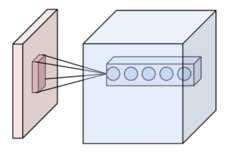
\includegraphics[scale=1.2]{figures/8.png}
	\caption{卷积核感受野及其输入和输出}
	\label{fig:f8}
\end{figure}

经过卷积层后,图像被抽象为新的形状和维度的特征图,通常被送进池化层进行池化操作,起到非线性降采样的作用。在保证平移不变性、尺度不变性等情况下,对图像不同位置的特征聚合统计,对卷积层输出的特征映射进行筛选过滤,压缩参数量,精简计算过程。一般所用到的池化方法有最大值池化和平均池化。池化层不需要学习参数,仅需要指定池化类型,池化操作核的大小和池化操作的步长即可。最大值池化每次操作时指定窗口大小,保留每个窗口中最大的数值,分别作用于输入特征图的各个通道,通道之间不会相互影响;平均池化是对邻域内特征点取平均。池化层的引入降低特征图的计算量,并具有一定的平移不变性,在整个过程中不会丢失重要信息,一定程度上可以降低网络模型训练时过拟合的概率,提升神经网络的泛化能力。在卷积神经网络架构中\textsuperscript{\cite{p10}},每个卷积层后面通常跟着一个激活函数,比如ReLU层,且通常会在连续的卷积层之间周期性地插入一个池化层。

此外卷积神经网络在训练的过程中,随着层层的提取,数据的分布会不断地变化并加以积累。故而在通常在网络中加以批归一化层来抑制中间层数据分布发生变化的情况。同时有效避免了网络收敛速度慢,梯度爆炸等情况,加速模型训练。

通常在卷积神经网络的最后会加以全连接层实现最终的分类等任务。可以将整个模型理解为通过层层全连接和池化层将原视信息映射到了一个隐空间,并通常由全连接层将特征映射到样本标签空间。

2012年Hinton等提出的AlexNet,以及2014年的VGG等便为经典的卷积神经网络模型。



\subsection{残差网络}{}

在2012年左的图像相关竞赛中,越来越深的神经网络模型依次展现了最好的表现。在网络层数的逐步加深时,深度残差网络可以说是近几年来计算机视觉及深度学习领域最具开创性的工作。残差结构使得网络可以训练到数百层且仍然具有较好的性能。

在图像相关的场景下,更深的网络意味着具有提取更多特征的可能性,故而堆叠越来越深的网络成为了一大趋势,用来丰富特征的维度。在网络层数的加深过程中时,虽然在一些场景下网络表现出了更高的精度和准确性,但也常常伴随着一些问题。例如梯度消失(Gradient Vanishing)和梯度爆炸(Gradient Exploding)。

当采用基于梯度的学习方法和反向传播来训练神经网络的时候,每一个神经网络的权值在每次训练迭代中接收一个与误差函数相对于当前权值的偏导数成比例的更新,此时浅层的偏导即为多个很小的偏导的乘积。当网络加深时,浅层的网络梯度便接近于0。而当梯度很小时,网络的学习速度极低,甚至完全阻止神经网络进行进一步的训练。如果该层网络的梯度一直很小,无法得到充分的训练,该层对整个网络便几乎不做贡献。类似地,当使用导数可以取较大值的激活函数时,则更易遇到爆炸梯度问题。

事实上,如图\ref{fig:f9}所示,实验表明,在进行传统的深度学习的训练过程中,随着ImageNet模型的网络层数的增加,最初越来越深的浅层网络的表现也越来越好,但当网络加深到一定阈值后,其准确率出现了退化(Degradation),训练误差越来越大。

\begin{figure}[h]
	\centering
	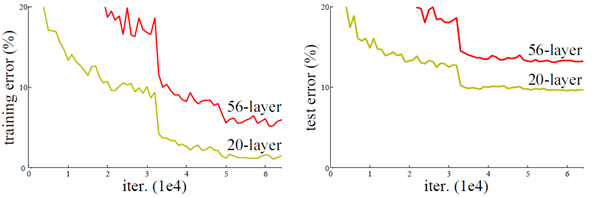
\includegraphics[scale=1]{figures/9.png}
	\caption{20层与56层的ImageNet网络误差\textsuperscript{\cite{p29}}}
	\label{fig:f9}
\end{figure}

解决梯度消失问题最有效的方法之一便是He等于2016年提出的残差神经网络,构建了跳跃连接来创建信息的“高速公路”,允许梯度信息通过各个层。其中前一层的输出被添加到更深一层的输出,这使得来自网络早期部分的信息可以被传递到网络的更深层部分,从而帮助在更深的网络中维持信号传播,对深层的网络重新引入浅层的输出来补偿消失的数据,同时解决了网络加深时的退化问题。

图\ref{fig:f10}为一个残差学习单元 (Residual Block),由两部分组成,右侧曲线为跳层连接的直接映射部分(Shortcut Connection),左侧曲线则包含卷积部分。

\begin{figure}[h]
	\centering
	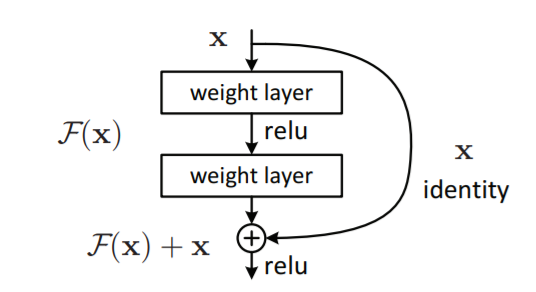
\includegraphics[scale=0.8]{figures/10.png}
	\caption{残差模块\textsuperscript{\cite{p29}}}
	\label{fig:f10}
\end{figure}

随着ResNet在研究领域的日益普及,其体系结构也得到了越来越多的研究,构造了许多基于ResNet的新体系结构。如Xie等人提出的一种ResNet的变体ResNeXt,其构建模块如图\ref{fig:f11}。

\begin{figure}[h]
	\centering
	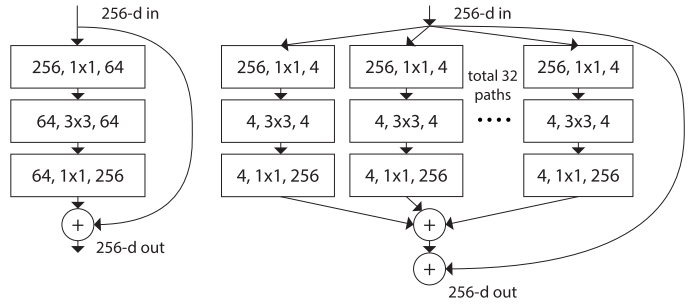
\includegraphics[scale=0.7]{figures/11.png}
	\caption{ResNeXt基本单元样例\textsuperscript{\cite{p28}}}
	\label{fig:f11}
\end{figure}

除此之外,Huang等人提出了一种名为DenseNet的新型架构。在ResNet中,跳跃连接主要是将距离较近的网络层之间进行连接,并让残差块串联组成整个网络来避免梯度消失和梯度爆炸以及网络的退化。DenseNet进一步利用了跳跃连接的效果,它使用跳跃连接,将所有神经网络层直接连接在一起。也就是说,对于每一层来说,其要处理的输入数据由在此之前全部的更浅层的特征图组成,其输出被传递到每个后续层。除了解决梯度消失的问题,这种架构同时支持了特性重用,使网络的参数效率大大提高。



\section{人体姿态描述模型}
本文的工作采用人体关节点坐标来描述人体的姿态。在human3.6m数据集中,人体关节点定义及编码如图\ref{fig:f12}所示:

0-Hip, 1-RightHip, 2-RightKnee, 3-RightAnkle, 4-RightSole, 5-RightToe, 6-LeftHip, 7-LeftKnee, 8-LeftAnkle, 9-LeftSole, 10-LeftToe, 11-Hip’, 12-Chest, 13-Neck, 14-Chin, 15-Head, 16-Neck’, 17-LeftShoulder, 18-LeftElbow, 19-LeftWrist, 20-LeftWrist’, 21-LeftOuterThigh, 22-LeftHand, 23-LeftHand’, 24-Neck’, 25-RightShoulder, 26-RightElbow, 27-RightWrist, 28-RightWrist’, 29-RightOuterThigh, 30-RightHand, 31-RightHand’

\begin{figure}[h]
	\centering
	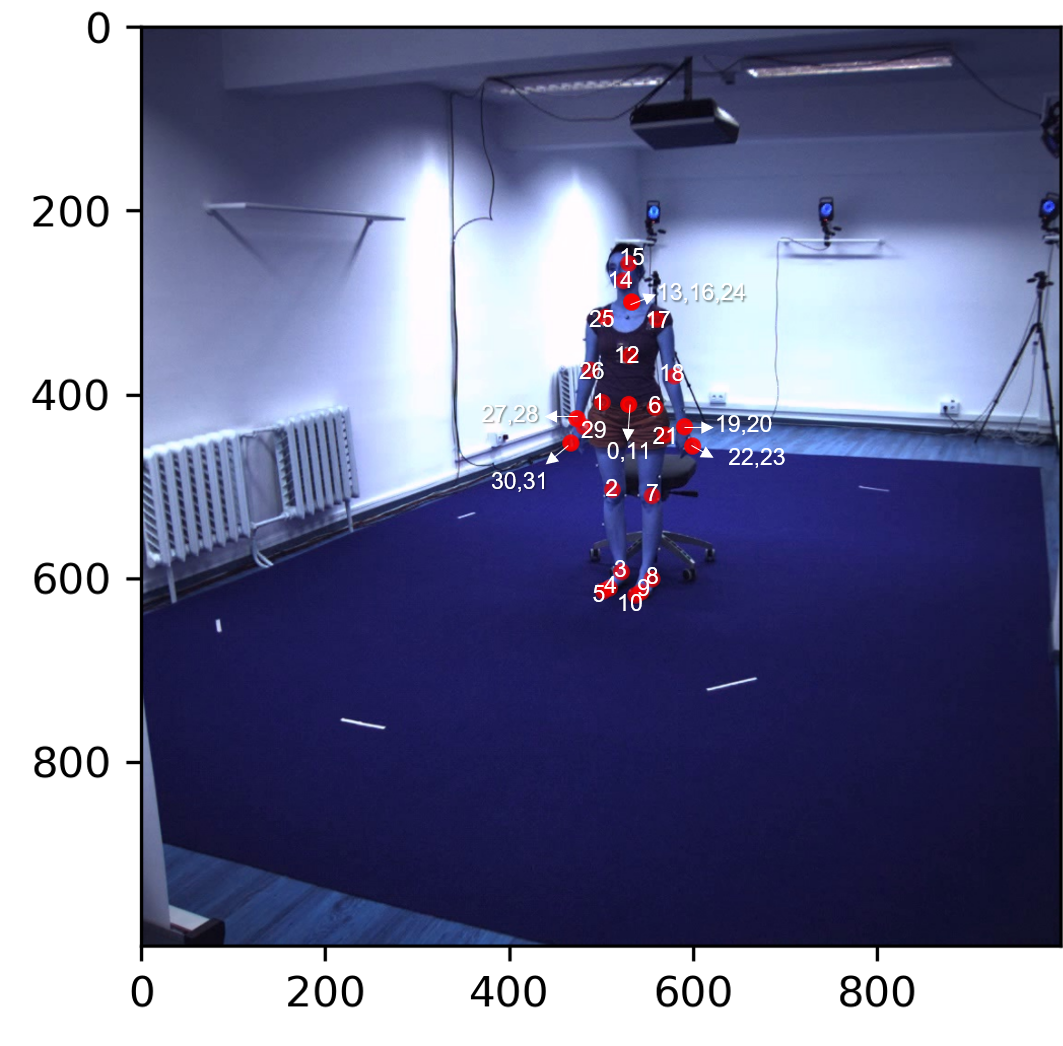
\includegraphics[scale=0.4]{figures/12.png}
	\caption{Human3.6m人体关节点标签及编码}
	\label{fig:f12}
\end{figure}


\section{动作捕捉}

\subsection{动作捕捉设备}{}
动作捕捉设备是运动物体的关键部位设置跟踪器。根据其技术原理分为惯性式、光感式等。并且由传感器、信号捕捉设备、数据传输设备与数据处理设备组成。

三维人体姿态数据的采集所需的动捕系统较为复杂,采集的数据格式与形式多样,以Human3.6m三维人体姿态数据集的采集系统为例。如图x所示,有4个数码摄像机,1个ToF时间飞行传感器和10 个动作捕捉相机共15个传感器。理论捕获区域大约为 6m x 5m,有效捕获区域大约 4m x 3m,在其中的对象对所有视频摄像机完全可见。

一组 10 个动作捕捉 (MX) 摄像机安装在墙壁上以最大化有效实验区域,左右边缘各 4 个,底部水平边缘大致中间 2 个。同时,还利用了Human Solutions (Vitus Smart LC3) 3D 激光人体扫描仪用于为参与实验的每个主体演员获得准确的 3D体积模型。

\begin{figure}[h]
	\centering
	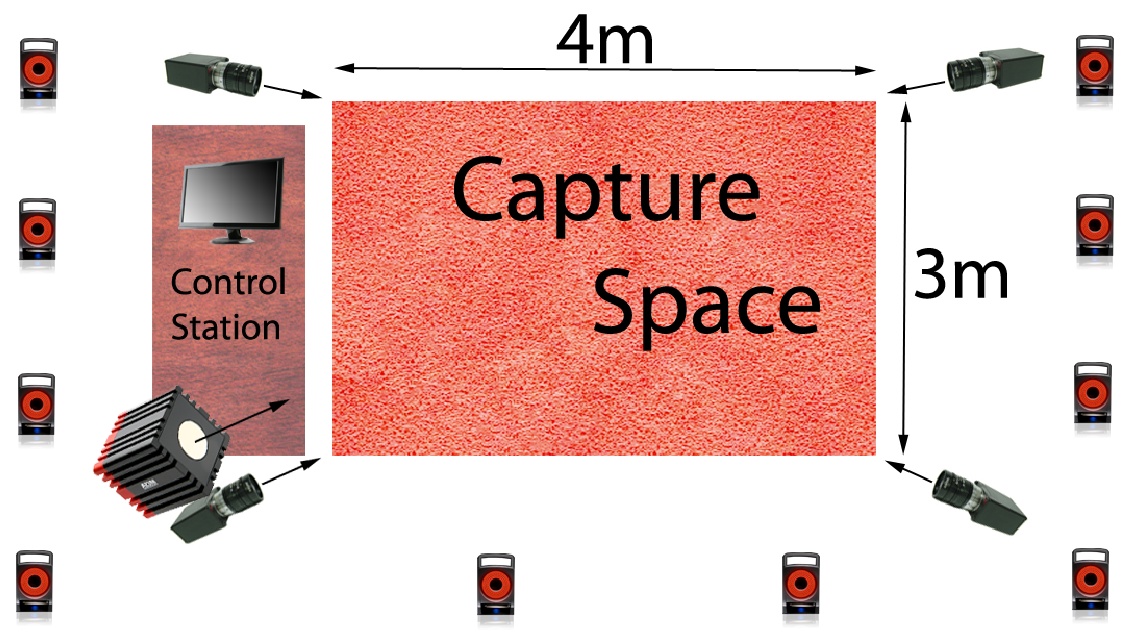
\includegraphics[scale=0.4]{figures/13.png}
	\caption{Human3.6m数据集采集区域\textsuperscript{\cite{p27}}}
	\label{fig:f13}
\end{figure}

数据集对以上各传感器的数据进行处理后,提供了各个相机的图像坐标系中的二维人体关节点坐标,三维人体关节点坐标,人体关节角度及人体三维扫描模型等。

而更为日常地,在普通的轻量级动作捕捉需求上,常见的惯性动作捕捉设备所采集的数据为bvh(Biovision hierarchical)文件格式\textsuperscript{\cite{p19}},仅记录了相应的人体骨架中各个骨骼或关节点的相对旋转角度。

\begin{figure}[h]
	\centering
	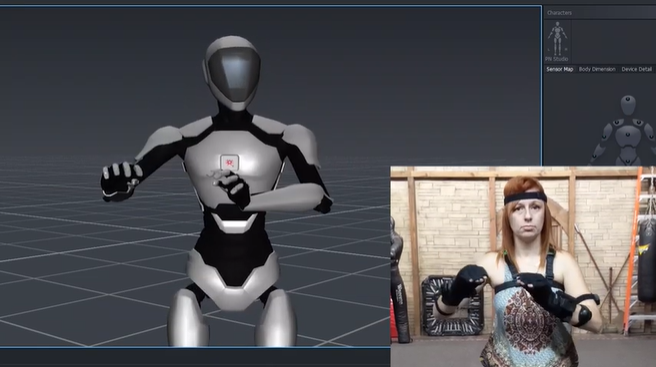
\includegraphics[scale=0.8]{figures/14.png}
	\caption{惯性动作捕捉设备及模型绑定效果}
	\label{fig:f14}
\end{figure}


\subsection{动作捕捉数据文件}{}
bvh(Biovision hierarchical data)是BioVision等动作捕捉设备对人体运动进行捕获后产生文件格式的文件扩展名\textsuperscript{\cite{p13}},同时可用于对其他角色骨的动作描述,如机器狗等。bvh文件主要记录了角色的骨骼树和其中的肢体关节在各帧中的旋转数据来描述运动。bvh 文件已经成为了一种通用的角色特征动画文件格式,MotionBuilder、3DMax等动画生成软件皆支持bvh文件的导入和编辑。

bvh文件由两部分组成,头部信息和之后的数据部分。bvh文件如图\ref{fig:f15}所示,头部信息首先包含了目标物体的各个关节点及其继承关系,同时包括了描述关节点运动的旋转和位移两种通道,以及默认骨骼模型中各个关节点相对于父节点的局部偏移量。最后,头部信息中还包含了文件描述的动作的帧数以及每帧时长,默认单位为秒。在bvh文件的数据部分,从第一帧开始,以深度优先遍历骨骼树的顺序依次对每个关节点的各个数据通道进行记录,直到最后一帧。

\begin{figure}[h]
	\centering
	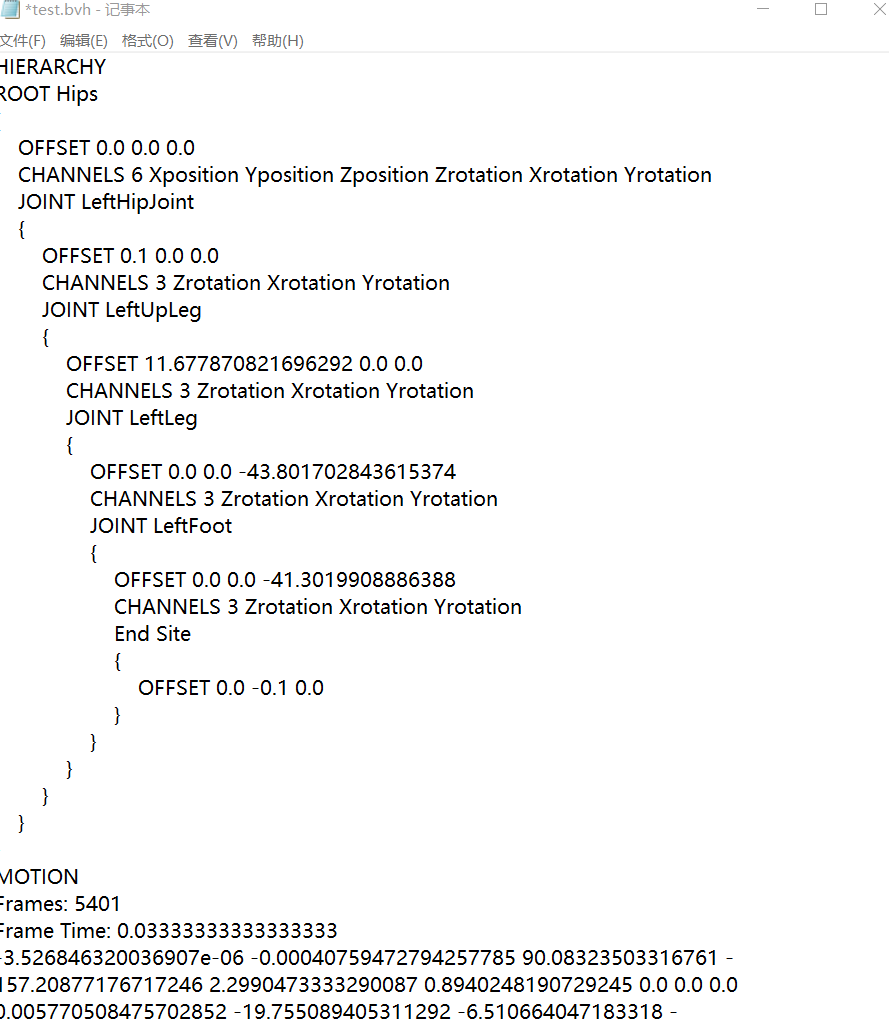
\includegraphics[scale=0.8]{figures/15.png}
	\caption{bvh文件样例}
	\label{fig:f15}
\end{figure}

更为具体的,HIERARCHY标记着关节继承信息描述的开始,ROOT为当前目标关节树唯一的根节点关节,JOINT指所有的子关节,OFFSET记录子关节相对于父关节的偏移量,CHANNELS表明数据记录部分对应的各个通道。特殊地,ROOT关节的通道中必须包含Xposition、Yposition、Zposition三个位移信息,而子节点的位移信息在具有rotation信息时为冗余数据,可以省略。

\subsection{欧拉角}{}
刚体运动(rigid motion)由旋转(rotation)和平移(translation)两部分组成,在描述人体的运动时,可以将人体抽象为由关节点组成的骨架,并将骨骼的运动近似为刚体运动。

对于已知的一次旋转变换,通常可以用旋转矩阵(Rotation matrix)来表示。而由于旋转矩阵有九个量,所以用它来描述只有三个自由度的一次旋转是冗余的。同时考虑到旋转矩阵具有行列式为1的正交矩阵的约束\textsuperscript{\cite{p18}},使得后续针对旋转矩阵的估计和优化较为困难。故而本文选择更为直观和简洁的欧拉角来对骨骼的旋转运动进行最终的描述和记录。

欧拉角的基本原理是记录目标绕一个轴旋转的角度,并将一次旋转分解为三次绕不同的轴的旋转,并规定绕三个轴旋转的次序以及旋转轴在之前的旋转中的固定与否。最终,欧拉角描述旋转的形态为一个三维向量。

通常,在欧拉角的描述过程中,利用了两个坐标系,固定不动的世界坐标系XYZ与随着物体的旋转而动的局部坐标系xyz。初始情况下,欧拉角描述的第一个旋转轴与世界坐标系的一个坐标轴一致。

假设局部坐标系与世界坐标系所形成的方向余弦矩阵(DCM, direction cosine matrix)已知,可得欧拉角。通常旋转顺序为Z-Y-X,物体先绕z轴旋转偏航角(yaw)的角度,再旋转之后的绕y轴旋转俯仰角(pitch),最后绕旋转之后的x轴旋转滚转角(roll)。
